\documentclass{beamer}
\usetheme{Malmoe}
\usecolortheme{seahorse}
\usepackage{pgfplots}
\usepackage{tikz}
\usetikzlibrary{datavisualization}
\usetikzlibrary{datavisualization.formats.functions}

\usepackage{textpos}
\usepackage{csquotes}
\usepackage{listings}
\usepackage{xurl}
\urlstyle{sf}
\usepackage{hyperref}
\usepackage{amsmath}
\usepackage{bm}
\usepackage{textcomp}
\usepackage{caption}
\usepackage{color}
\usepackage{subfigure}
\usepackage{wrapfig}
\usepackage[english,ngerman]{babel}
\usepackage[backend=biber,style=alphabetic]{biblatex}
\usepackage{mathtools}
\usepackage{subdepth}
\usepackage{graphicx}
\usepackage{blindtext}
\usepackage{svg}
\usepackage{xcolor,colortbl}
\usepackage{media9}

\let\oldcite=\cite
\renewcommand{\cite}[1]{\textcolor[rgb]{.55,.55,.89}{\oldcite{#1}}}

\setbeamerfont{frametitle}{size=\small}
\addbibresource{../mscthesis.bib}
\addbibresource{pres.bib}
\captionsetup{justification=raggedright,singlelinecheck=false}
\DeclareMathOperator*{\argmin}{arg min}
\makeatletter
\def\ext@algorithm{lol}% algorithm captions will be written to the .lol file
% share the list making commands and redefine the heading
\AtBeginDocument{%
  \let\l@algorithm\l@lstlisting
  \let\c@algorithm\c@lstlisting
  \let\thealgorithm\thelstlisting
  \renewcommand{\lstlistlistingname}{Algorithms and source code}%
}
\makeatother
\lstdefinelanguage{GLSL}
{
  sensitive=true,
  morekeywords=[1]{
    attribute, const, uniform, varying,
    layout, centroid, flat, smooth,
    noperspective, break, continue, do,
    for, while, switch, case, default, if,
    else, in, out, inout, float, int, void,
    bool, true, false, invariant, discard,
    return, mat2, mat3, mat4, mat2x2, mat2x3,
    mat2x4, mat3x2, mat3x3, mat3x4, mat4x2,
    mat4x3, mat4x4, vec2, vec3, vec4, ivec2,
    ivec3, ivec4, bvec2, bvec3, bvec4, uint,
    uvec2, uvec3, uvec4, lowp, mediump, highp,
    precision, sampler1D, sampler2D, sampler3D,
    samplerCube, sampler1DShadow,
    sampler2DShadow, samplerCubeShadow,
    sampler1DArray, sampler2DArray,
    sampler1DArrayShadow, sampler2DArrayShadow,
    isampler1D, isampler2D, isampler3D,
    isamplerCube, isampler1DArray,
    isampler2DArray, usampler1D, usampler2D,
    usampler3D, usamplerCube, usampler1DArray,
    usampler2DArray, sampler2DRect,
    sampler2DRectShadow, isampler2DRect,
    usampler2DRect, samplerBuffer,
    isamplerBuffer, usamplerBuffer, sampler2DMS,
    isampler2DMS, usampler2DMS,
    sampler2DMSArray, isampler2DMSArray,
  usampler2DMSArray, struct},
  morekeywords=[2]{
    radians,degrees,sin,cos,tan,asin,acos,atan,
    atan,sinh,cosh,tanh,asinh,acosh,atanh,pow,
    exp,log,exp2,log2,sqrt,inversesqrt,abs,sign,
    floor,trunc,round,roundEven,ceil,fract,mod,modf,
    min,max,clamp,mix,step,smoothstep,isnan,isinf,
    floatBitsToInt,floatBitsToUint,intBitsToFloat,
    uintBitsToFloat,length,distance,dot,cross,
    normalize,faceforward,reflect,refract,
    matrixCompMult,outerProduct,transpose,
    determinant,inverse,lessThan,lessThanEqual,
    greaterThan,greaterThanEqual,equal,notEqual,
    any,all,not,textureSize,texture,textureProj,
    textureLod,textureOffset,texelFetch,
    texelFetchOffset,textureProjOffset,
    textureLodOffset,textureProjLod,
    textureProjLodOffset,textureGrad,
    textureGradOffset,textureProjGrad,
    textureProjGradOffset,texture1D,texture1DProj,
    texture1DProjLod,texture2D,texture2DProj,
    texture2DLod,texture2DProjLod,texture3D,
    texture3DProj,texture3DLod,texture3DProjLod,
    textureCube,textureCubeLod,shadow1D,shadow2D,
    shadow1DProj,shadow2DProj,shadow1DLod,
    shadow2DLod,shadow1DProjLod,shadow2DProjLod,
    dFdx,dFdy,fwidth,noise1,noise2,noise3,noise4,
  EmitVertex,EndPrimitive},
  morekeywords=[3]{
    gl_VertexID,gl_InstanceID,gl_Position,
    gl_PointSize,gl_ClipDistance,gl_PerVertex,
    gl_Layer,gl_ClipVertex,gl_FragCoord,
    gl_FrontFacing,gl_ClipDistance,gl_FragColor,
    gl_FragData,gl_MaxDrawBuffers,gl_FragDepth,
    gl_PointCoord,gl_PrimitiveID,
    gl_MaxVertexAttribs,gl_MaxVertexUniformComponents,
    gl_MaxVaryingFloats,gl_MaxVaryingComponents,
    gl_MaxVertexOutputComponents,
    gl_MaxGeometryInputComponents,
    gl_MaxGeometryOutputComponents,
    gl_MaxFragmentInputComponents,
    gl_MaxVertexTextureImageUnits,
    gl_MaxCombinedTextureImageUnits,
    gl_MaxTextureImageUnits,
    gl_MaxFragmentUniformComponents,
    gl_MaxDrawBuffers,gl_MaxClipDistances,
    gl_MaxGeometryTextureImageUnits,
    gl_MaxGeometryOutputVertices,
    gl_MaxGeometryOutputVertices,
    gl_MaxGeometryTotalOutputComponents,
    gl_MaxGeometryUniformComponents,
  gl_MaxGeometryVaryingComponents,gl_DepthRange},
  morecomment=[l]{//},
  morecomment=[s]{/*}{*/},
  morecomment=[l][keywordstyle4]{\#},
}
\lstdefinestyle{GL}{
  tabsize=2,
  rulecolor=,
  basicstyle=\scriptsize,
  upquote=true,
  aboveskip={0.5\baselineskip},
  belowskip={1.5\baselineskip},
  columns=fixed,
  showstringspaces=false,
  extendedchars=true,
  breaklines=true,
  prebreak = \raisebox{0ex}[0ex][0ex]{\ensuremath{\hookleftarrow}},
  frame=single,
  showtabs=false,
  showspaces=false,
  showstringspaces=false,
  identifierstyle=\ttfamily,
  keywordstyle=\color[rgb]{1.0,0,0},
  keywordstyle=[1]\color[rgb]{0,0,0.75},
  keywordstyle=[2]\color[rgb]{0.5,0.0,0.0},
  keywordstyle=[3]\color[rgb]{0.127,0.427,0.514},
  keywordstyle=[4]\color[rgb]{0.4,0.4,0.4}}

\setcounter{biburllcpenalty}{7000}
\setcounter{biburlucpenalty}{8000}

%Information to be included in the title page:


\title{GPU Acceleration of the Material Point Method}

\author % (optional, for multiple authors)
{Fabian Meyer}

\institute % (optional)
{University of Koblenz}

\date{Kolloquium Computergrafik, 14 February 2019}

\begin{document}
\begin{frame}
\titlepage
\end{frame}

\section{Motivation on a GPU MPM Approach}

\subsection{A Brief MPM Overview: Do You Want to Build a Snowman?}

\begin{frame}

\frametitle{A Brief MPM Overview: Do You Want to Build a Snowman?}
A short historical summary of MPM:
\vfill
\begin{minipage}{0.43\paperwidth}
  \begin{itemize}
    \item Belongs to family of particle-in-cell(PIC) techniques \cite{evans1957particle}.
    \item Initial application to solids \cite{sulsky1995application} $\rightarrow$ MPM
    \item From research to production in \textit{Disney's} animation film \textit{Frozen} \cite{MPM:SNOW}.
    \item Avalanche research \cite{MPM:AVALANCHE}
  \end{itemize}
\end{minipage}
\begin{minipage}{0.35\paperwidth}
\includemedia[
  width=144,
  height=81,
  activate=pageopen,
  addresource=media/snowh264.mp4,
  flashvars={source=media/snowh264.mp4&autoPlay=true&loop=true&repeat=always}
  ]{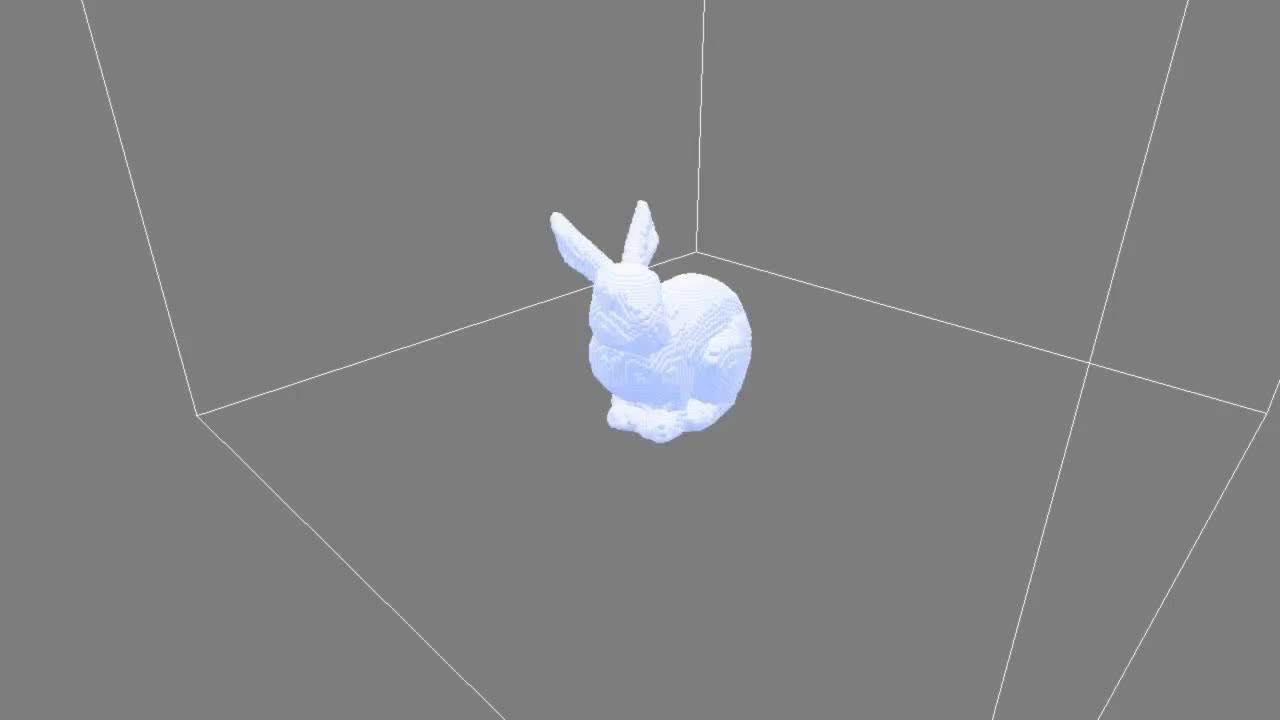
\includegraphics{media/snow.jpg}}{VPlayer.swf}
  \tiny{Video result of my bachelor thesis on the simulation of snow \cite{Meyer2015}.}
\end{minipage}
\end{frame}


\begin{frame}
PIC ideas:
\vfill
\begin{minipage}{0.45\paperwidth}
\begin{itemize}
    \item Combine Lagrangian particles \& Eulerian grid    \item Particles store all information
\end{itemize}
\vfill
Typical PIC/MPM roundtrip:
\vfill
\begin{enumerate}
  \item Particle-to-grid(P2G) transfer to an unmoving grid
    \item Solve discretized governing equations on grid
    \item Grid-to-particle(G2P) transfer back to particles \& move them
    \item[$\Rightarrow$] \textbf{meshfree, non-empirical}
\end{enumerate}
\end{minipage}
\begin{minipage}{0.35\paperwidth}
	\includesvg[width=0.35\paperwidth]{media/pic.svg}
	\tiny{Transfers: Interpolation functions are defined over grid nodes.}
\end{minipage}
\end{frame}
\subsection{GPGPU for performance enthusiasts}
\begin{frame}
  \frametitle{GPGPU for performance enthusiasts}
  Why would('nt) you?
  \vfill
  \begin{columns}[T]
    \begin{column}{0.45\textwidth}
      \textbf{Drawbacks:}
    \begin{itemize}
      \item Interactivity much easier on CPU, but slow PCI-Bus communication
      \item Code is mostly written against GPU architecture
      \item A lot of strain on the programmer
    \end{itemize}
    \end{column}
    \begin{column}{0.45\textwidth}
      \textbf{Benefits:}
    \begin{itemize}
      \item Data is already on the GPU for rendering
      \item \textbf{Higher parallelization acceleration}
    \end{itemize}
    \end{column}
  \end{columns}
\end{frame}
\section{A Gentle Introduction to the MPM}


\subsection{Governing Equations: Conservation of Mass \& Momentum}

\begin{frame}
  \frametitle{Governing Equations: Conservation of Mass \& Momentum}
  \textbf{Conservation of mass}, continuum assumption holds.\\
  Lagrangian (moving with a particle ${}_0\boldsymbol{x}$):
  \begin{equation}
    {^t_0J}\rho(_0\boldsymbol{x},t) = {}\rho(_0\boldsymbol{x},0).
  \end{equation}
Eulerian (outside observer ${}_t\boldsymbol{x}$):
\begin{equation}
  \frac{\partial}{\partial t}\rho(_t\boldsymbol{x},t) = -  \vec{\nabla} \cdot (\rho(_t\boldsymbol{x},t) \boldsymbol{v}(_t\boldsymbol{x},t)).
\end{equation}
Lagrangian and Eulerian view measure differently but give same results. Equations are given in the strong form! \cite{MPM:COURSE}\cite{MIT:CONTINUUM_MECHANICS}
\end{frame}

\begin{frame}
  \textbf{Conservation of momentum}:\\
  Lagrangian (moving with a particle ${}_0\boldsymbol{x}$):
  \begin{equation}
  \rho(_0\boldsymbol{x},0)\boldsymbol{a}(_0\boldsymbol{x},t)
= \vec{\nabla} \cdot \boldsymbol{P}(_0\boldsymbol{x},t) + {\boldsymbol{f}} ^ {\text{body}}(_0\boldsymbol{x},t) {^t_0J}.
  \end{equation}
Eulerian (outside observer ${}_t\boldsymbol{x}$):
\begin{equation}
  \rho(_t\boldsymbol{x},t) \boldsymbol{a}(_t\boldsymbol{x},t) = \vec{\nabla} \cdot \boldsymbol{\sigma}(_t\boldsymbol{x},t) + \boldsymbol{f} ^ {\text{body}}(_t\boldsymbol{x},t)
\end{equation}
Solving this equation will tell us how the velocity fields $\boldsymbol{v}(_t\boldsymbol{x}),\boldsymbol{v}(_0\boldsymbol{x})$ change on the whole domain due to acceleration $\boldsymbol{a}$. This is important to advect particles accounting for all forces. \cite{MPM:COURSE}\cite{MIT:CONTINUUM_MECHANICS}
\end{frame}

\subsection{The Pretty Strong but Mathematically Weak Formulation}
\begin{frame}
\frametitle{The Pretty Strong but Mathematically Weak Formulation}

\textbf{Weak Formulation} (or Principle of Virtual Work):\\
Dot product equations with arbitrarily 'test functions' $\boldsymbol{q}$ and apply divergence theorem:
\begin{align}
\int _ { \Omega ^ { 0 } } _0\boldsymbol{q} \cdot  \Bigl[(_0\rho_0)(_0\boldsymbol{a}) - & {}_0\boldsymbol{f}^{\text{body}}{}_0^tJ\Bigr] d _0\boldsymbol{x}= \nonumber \\
										     &  \int _ { \partial \Omega ^ { t^n } } _t\boldsymbol{q} \cdot \boldsymbol{\sigma} d_t\boldsymbol{A} - \int _ { \Omega ^ { t^n} } \nabla {}_t\boldsymbol{q} : \boldsymbol{\sigma}  d_t\boldsymbol{x}.
\end{align}
A strong solution is also a solution to the weak formulation. Leave out body forces(like gravity) and boundary condition (e.g. collisions) for now:
\begin{equation}
  \int _ { \Omega ^ { 0 } } _0\boldsymbol{q} \cdot (_0\rho_0)(_0\boldsymbol{a}) d _0\boldsymbol{x}= \int _ { \Omega ^ { t^n} } \nabla {}_t\boldsymbol{q} : \boldsymbol{\sigma}  d_t\boldsymbol{x}.
\end{equation}
\end{frame}
\begin{frame}[fragile]
\textbf{Weak Derivative}:
\vfill
\begin{minipage}{0.49\textwidth}
  $y=|t|$ has weak derivative:
  \\\\
$ v = \left\{ \begin{array} { l l }
{ - 1 , } & { \text { if } t < 0 } \\
{ c , } & { \text { if } t = 0 } \\
{ 1 , } & { \text { if } t > 0 }
\end{array} \right.$
\\

\end{minipage}
\begin{minipage}{0.4\textwidth}
\begin{tikzpicture}
\datavisualization [school book axes,
		    visualize as line/.list={fx},
		    fx={style={color=blue}}
]

data [set=fx,format=function] {
      var x : interval [-1.5:1.5] samples 5;
      func y = abs(\value x);
      };
\end{tikzpicture}
\end{minipage}

\vfill
\begin{minipage}{0.49\textwidth}
  Heaviside step function has no weak derivate: \\\\
  $y= \left\{ \begin{array} { l l } { 0 , } & { \text { if } t < 0 } \\ { 1 , } & { \text { if } t \geq 0 } \end{array} \right.$
\end{minipage}
\begin{minipage}{0.4\textwidth}


\begin{tikzpicture}

  \datavisualization [school book axes,
		      visualize as line/.list={fx},
		      fx={style={color=blue}}]
data[set=fx] {
  x, y
  -1.5, 0
  0, 0
  0, 1
  1.5, 1
};
\end{tikzpicture}
\end{minipage}
\vfill
Allows for point loads, material discontinuities and more. \cite{bathe2006finite}
\end{frame}
\subsection{Discretization of Space and Time}
\begin{frame}
\frametitle{Discretization of Space and Time}
\textbf{Time discretization} with implicit midpoint scheme:
  \begin{equation}
    \frac { y ^ { n + 1 } - y ^ { n } } { \Delta t } = f ^ { n + \frac{1}{2} } = f \left( t ^ { n } + \frac{\Delta t}{2}, \frac{1}{2} y ^ { n } + \frac{1}{2} y ^ { n + 1 } \right)
  \end{equation}
\begin{itemize}
  \item \textbf{implicit} requires linear system solve $\Rightarrow$ more stable, larger time steps
  \item \textbf{midpoint} as it conserves gov. equations
\end{itemize}

  \begin{equation}
    \Rightarrow \int _ { \Omega ^ { t } } _t\boldsymbol{q} \cdot {}_t\rho(_t\boldsymbol{v}^{n+1}-{}_t\boldsymbol{v}^{n}) d _t\boldsymbol{x}= \int _ { \Omega ^ { t^n} } \nabla {}_t\boldsymbol{q} : \boldsymbol{\sigma}^{n+\frac{1}{2}}  d_t\boldsymbol{x}.
  \end{equation}
\end{frame}

\begin{frame}[fragile]
\textbf{Space Discretization} is done in a Galerkin/FEM fashion with grid based interpolants $w_i$ with limited support. Here dyadic products
\begin{equation}
  w_i(\boldsymbol{x}) =w(\boldsymbol{x}-\boldsymbol{x}_i) = w(\frac{1}{h}(x-x_i))w(\frac{1}{h}(y-y_i)w(\frac{1}{h}(z-z_i))
\end{equation}
of cubic b-splines suffice:
\begin{equation}
w ( x ) = \left\{ \begin{array} { l l } { \frac { 1 } { 2 } | x | ^ { 3 } - | x | ^ { 2 } + \frac { 2 } { 3 } } & { 0 \leqslant | x | < 1 } \\ { \frac { 1 } { 6 } ( 2 - | x | ) ^ { 3 } } & { 1 \leqslant | x | < 2 } \\ { 0 } & { 2 \leqslant | x | } \end{array}. \right
\end{equation}
\end{frame}
\begin{frame}

\begin{tikzpicture}[domain=0:1]
\begin{axis}
\addplot {x*x};
\end{axis}
\end{tikzpicture}

\end{frame}
\begin{frame}
Thus set in:
$$
{}_t\boldsymbol{q}(\boldsymbol{x},t^n) = \sum_i \boldsymbol{e}_iw_i(\boldsymbol{x}),
{}_t\boldsymbol{v}^{n(+1)}(\boldsymbol{x}) = \sum_j \boldsymbol{v}^{n(+1)}_jw_j(\boldsymbol{x}).
$$
Combine it with Numerical Integration where the particles function as quadrature points:
\end{frame}
\section{A MPM Guide on GPGPU Pitfalls and Optimizations}
\subsection{d}

\begin{frame}
\frametitle{hi}
  \begin{enumerate}
    \item \cite{MPM:COURSE}
  \end{enumerate}
\end{frame}

\section{Delving Deeper: Further Opportunities}

\subsection{d}

\begin{frame}
\frametitle{hi}
  \begin{enumerate}
    \item \cite{MPM:COURSE}
  \end{enumerate}
\end{frame}

\selectlanguage{english}
\printbibliography
\end{document}
